\documentclass[fancy, masters,twoside]{byuthesis}
% Class options are simple/fancy and masters/phd.
% Leave options blank for defaults.
% Defaults are simple for document style, and masters for degree type.


%%%%%%%%%%%%%%%%%%%%%%%%%%%%%%%
% Custom options and packages %
%%%%%%%%%%%%%%%%%%%%%%%%%%%%%%%
% Define path to figure files
\graphicspath{{figures/}}

% Define sequences of Latin text to fill space in example documents
% (not needed for your thesis -- delete or comment out if you'd like)
\usepackage{blindtext}


%%%%%%%%%%%%%%%%%%%%%%%%%%%%%%
% Define title page elements %
%%%%%%%%%%%%%%%%%%%%%%%%%%%%%%
% Thesis title for required BYU title page
\title{Evaluating Parameter Uncertainty in Transportation\\
Demand Models}

% On the custom title page, use the same title, but format as you like
\customtitle{Evaluating Parameter Uncertainty in Transportation\\
Demand Models}

% Your name goes here:
\author{Natalie Mae Gray}

% This is the date of graduation
\date{April 2021}

% If your degree is not a PhD or MS, then you can overwrite the degree using
\degree{Master of Science}

% Your department
\department{Department of Civil and Construction Engineering}

% The names of your committee members
\committeechair{Gregory S. Macfarlane}
  \committeemember{Grant G. Schultz}
  \committeemember{Daniel P. Ames}

% Include any keywords you would like for your thesis/dissertation
\keywords{sensitivity analysis, transportation demand model, transportation planning, latin hypercube sampling, monte carlo simulation}


%%%%%%%%%%%%%%%%%%%%%%%%%%%%%%%%%%
% ---Bibliography source file--- %
%%%%%%%%%%%%%%%%%%%%%%%%%%%%%%%%%%
	\usepackage{booktabs}
\usepackage{longtable}
\usepackage{array}
\usepackage{multirow}
\usepackage{wrapfig}
\usepackage{float}
\usepackage{colortbl}
\usepackage{pdflscape}
\usepackage{tabu}
\usepackage{threeparttable}
\usepackage{threeparttablex}
\usepackage[normalem]{ulem}
\usepackage{makecell}
\usepackage{xcolor}


%%%%%%%%%%%%%%%%%%%%%%%%%%%%%%%%%%
% ---Bibliography source file--- %
%%%%%%%%%%%%%%%%%%%%%%%%%%%%%%%%%%
%  Default is references.bib
%
\makepagestyle{myrefs}
\makeevenhead{myrefs}%
    {\normalfont\small\slshape\thepage}{}{\normalfont\small\slshape References}
\makeoddhead{myrefs}%
    {\normalfont\small\slshape References}{}{\normalfont\small\slshape\thepage}
\bibliography{}

\newlength{\cslhangindent}
\setlength{\cslhangindent}{1.5em}
\newlength{\csllabelwidth}
\setlength{\csllabelwidth}{3em}
\newlength{\cslentryspacingunit} % times entry-spacing
\setlength{\cslentryspacingunit}{\parskip}
% for Pandoc 2.8 to 2.10.1
\newenvironment{cslreferences}%
  {}%
  {\par}
% For Pandoc 2.11+
\newenvironment{CSLReferences}[2] % #1 hanging-ident, #2 entry spacing
 {% don't indent paragraphs
  \setlength{\parindent}{0pt}
  % turn on hanging indent if param 1 is 1
  \ifodd #1
  \let\oldpar\par
  \def\par{\hangindent=\cslhangindent\oldpar}
  \fi
  % set entry spacing
  \setlength{\parskip}{#2\cslentryspacingunit}
 }%
 {}
\usepackage{calc}
\newcommand{\CSLBlock}[1]{#1\hfill\break}
\newcommand{\CSLLeftMargin}[1]{\parbox[t]{\csllabelwidth}{#1}}
\newcommand{\CSLRightInline}[1]{\parbox[t]{\linewidth - \csllabelwidth}{#1}\break}
\newcommand{\CSLIndent}[1]{\hspace{\cslhangindent}#1}

\providecommand{\tightlist}{%
  \setlength{\itemsep}{0pt}\setlength{\parskip}{0pt}}

%%%%%%%%%%%%%%%%%%%%%%%%%%
% --- Begin Document --- %
%%%%%%%%%%%%%%%%%%%%%%%%%%
\begin{document}


%%%%%%%%%%%%%%%%%%%%%%%%%%%%%%%%%%%%%%%%%%%%%%%%%%%%%%%
% --- Front matter (probably don't need to change)--- %
%%%%%%%%%%%%%%%%%%%%%%%%%%%%%%%%%%%%%%%%%%%%%%%%%%%%%%%
	\frontmatter

	\titlepage
	\cleardoublepage

	\customtitlepage
	\cleardoublepage


    \begin{abstract}
  \textbf{\emph{NEED}} The abstract of a thesis should describe the
  motivation, objective, overall results, and central findings of the thesis.
  It may have multiple paragraphs if necessary.
  \end{abstract}
  	\cleardoublepage


    \begin{acknowledgments}
  \textbf{\emph{NEED}} Students should acknowledge funding sources. They may also use the
  acknowledgment page to express appreciation for the committee members, friends
  or family who provided assistance in research, writing or technical aspects of
  the dissertation, thesis or selected project. Acknowledgements should be simple
  and in good taste.
  \end{acknowledgments}
  	\cleardoublepage

	\tableofcontents*
	\cleardoublepage

	\listoffigures
	\cleardoublepage

	\listoftables
	\cleardoublepage

	\nomenclature{$c$}{Speed of light in a vacuum inertial frame}
\nomenclature{$h$}{Planck constant}
\nomenclature{$\mathit{Re}$}{Reynolds number}
\nomenclature{$\mathbf{x}$}{State vector}
\nomenclature{$\alpha$}{Angle of attack}
\nomenclature{$\beta$}{Sideslip angle}
\nomenclature{$\gamma$}{Climb angle}
\nomenclature{$p$}{Roll rate}
\nomenclature{$q$}{Pitch rate}
\nomenclature{$r$}{Yaw rate}
\nomenclature{$P$}{Covariance matrix}

\printnomenclature
	\cleardoublepage

%%%%%%%%%%%%%%%%%%%%%
% --- Main Body --- %
%%%%%%%%%%%%%%%%%%%%%
	\mainmatter

\hypertarget{introduction}{%
\chapter{Introduction}\label{introduction}}

\hypertarget{problem-statement}{%
\section{Problem Statement}\label{problem-statement}}

The inherent accuracy and uncertainty in travel forecasting models is receiving increasing attention from the scholarly and practicing community. Given that such models are used in the allocation of billions of dollars of infrastructure financing each year, the financial risks for inaccurate or imprecise forecasts are high (Flyvbjerg et al., 2005; Voulgaris, 2019; Wu \& Levinson, 2021).

Transportation demand forecasting models, like other mathematical-statistical models, might be abstracted to the following basic form,
\begin{equation}
y = f(X, \beta)
\end{equation}
where \(y\) is the variable being predicted based on input data \(X\), moderated through a specific functional form \(f()\) and parameters \(\beta\). Three sources of error may lead a forecast value \(\hat{y}\) to differ from the ``true'' or ``actual'' value of \(y\) (Rasouli \& Timmermans, 2012):

\begin{enumerate}
\def\labelenumi{\arabic{enumi}.}
\item
  The input data \(X\) might contain errors, due to inaccuracies in the base year, or an inaccurate projection of land use, petroleum price, or other key input variable. This was the primary issue identified by (Hoque et al., 2021) in a historical analysis of the accuracy of travel forecasts.
\item
  The model form \(f()\) may be improperly specified. Variables that play a major role in travel behavior may not be included due to lack of information, or the unobserved error components may have a different correlation than was assumed during model development. A detailed description of specifying mode choice model variables and nesting of error structures is given by Koppelman \& Bhat (2006).
\item
  The parameter estimates \(\hat{\beta}\) may have incorrect values. This may be because the parameters were estimated on an improperly specified model \(f()\), or because the estimation dataset was improperly weighted.
\end{enumerate}

Of these potential sources of error, only the third is addressed in classical statistics. The standard errors of the model parameter estimates in a theoretical perspective address the uncertainty question to a great degree. Yet even this source of uncertainty has been largely ignored in transportation forecasts, and model development documentation often elides these values completely (National Academies of Sciences et al., 2012). Zhao \& Kockelman (2002) examined the effects of this parameter uncertainty in a contrived 25 zone trip-based model, but a systemic analysis of this uncertainty in a practical model is not common.

\hypertarget{objectives}{%
\section{Objectives}\label{objectives}}

In this research, we investigate the uncertainty in traffic forecasts resulting from plausible uncertainty in an advanced trip-based transportation demand model. Using a Latin hypercube sampling (LHS) methodology, we simulate one hundred potential parameter sets for a combined mode and destination choice model in Roanoke, Virginia, USA. We then assign the resulting trip matrices to the highway network for the region and evaluate the PM and daily assigned traffic volumes alongside the variation in implied impedance and accessibility.

This paper proceeds first with a literature review in Chapter 2, followed by a description of the model design and simulation sampling methodology in Chapter 3, succeeded by a discussion of the variation in mode, destination, and traffic performance measures in Chapter 4. The paper concludes in Chapter 5 with a summary of the key findings alongside a presentation of limitations and related indications for future research.

\hypertarget{literature-review}{%
\chapter{Literature Review}\label{literature-review}}

\hypertarget{overview}{%
\section{Overview}\label{overview}}

Researchers acknowledge that there exists uncertainty in transportation demand models, though few choose to quantify it. This review looks at the types of uncertainty that exists, and research that has been done to evaluate uncertainty.

\hypertarget{types-of-uncertainty}{%
\section{Types of Uncertainty}\label{types-of-uncertainty}}

Uncertainty generally exists from two basic sources: input uncertainty and model uncertainty (Rasouli \& Timmermans, 2012). Input uncertainty includes behavioral and socioeconomic data -- for instance, the number of jobs and residents in a zone might be coded incorrectly -- as well as parameter estimates including automobile operating costs, gasoline costs, and values of time. Model uncertainty can be further divided into specification error and estimation error. Specification error is a failure to estimate the ``true'' model. Estimation error, on the other hand, is a failure to estimate the correct values of model constants and parameters, or taking the mean estimated value as a single parameter. Previous research exits to identify and quantify each of these sources of error. An overview of the literature and which source of uncertainty they evaluate can be found in Table \ref{tab:authors}.

Rodier \& Johnston (2002) looked at uncertainty in socioeconomic projections (population and employment, household income, and fuel prices) at the county-level for the Sacramento, California region. They wanted to know if the uncertainty in the range of plausible socioeconomic values were a significant source of error in the projection of future travel patterns and vehicle emissions. They identified ranges for population and employment, household income, and fuel price for two scenario years (2005 and 2015). The ranges varied based on the scenario year and the socioeconomic variable. They changed one variable at a time for a total of 19 iterations of the model run for 2005 and 21 iterations for 2015. Their results indicated that the error in projections for household income and fuel prices is not a significant source of uncertainty, but error ranges for population and employment projections are a significant source for changes in travel and emissions.

Zhao \& Kockelman (2002) looked at the propagation of uncertainty through each step of their transportation demand model from variation among inputs and parameters. This analysis used a traditional four-step urban transportation planning process (trip generation, trip attraction, mode split, and trip assignment) on a 25-zone sub-model of the Dallas-Fort Worth metropolitan region. Monte Carlo simulation was used to vary the input and parameter values. These values were all ranged using a coefficient of variation (cov) of 0.30, with the inputs only in the positive direction. The four-step model was ran 100 times with 100 different sets of input and parameter values. The results of these runs showed that uncertainty increased in the first three steps of the model and the final assignment step reduced the compounded uncertainty, although not below the levels of input uncertainty. Uncertainty propagation was found to be significant from changes in inputs and parameters, but the final step nearly stabilizes the uncertainty to the same amount as assumed (0.30 cov assumption with a 0.31 cov in the results of trip assignment).

Clay \& Johnston (2005) varied three inputs and one parameter to analyze uncertainty of outputs on a fully integrated land use and travel demand model of six counties in the Sacramento, California region. The variales used for analysis were exogenous production, commercial trip generation rates, perceived out-of-pocket costs of travel for single occupant vehicles, and concentration parameter. Exogenous production, commercial trip generation rates, and the concentration parameter were varied by plus or minus 10, 25 and 50\%, while the cash cost of driving was varied by plus or minus 50 and 100\%. This resulted in 23 model runs, one for each changed variable and one for the base scenario. Their research found that any uncertainty in the inputs resulted in large difference in the VMT output, although this difference was a lower percentage than the uncertainty in the input.

Flyvbjerg et al. (2005) researched the specification error of various forecasting traffic models. They used the forecast data for a given year and the actual value that was collected for the same year. Their study found that there is a statistical significance in the difference of the estimated and actual values. Rail projects are generally overestimate passenger forecasts by 106\%, and half of road projects have a traffic forecast difference of plus or minus 20\%. They did not identify where this inaccuracy came from, but they identified that it was important for future research.

Armoogum et al. (2009) looked at uncertainty within an age-cohort forecasting model for the Paris and Montreal metropolitan regions. The sources of uncertainty analysed were calibration of the model, behavior of future generations, and demographic projections. A jackknife technique was used to estimated confidence intervals for each source of error using multiple years of analysis. They found that the longer the forecasting period was, the larger the uncertainty. Generally the model foretasted within 10-15\%, reaching higher percentage ranges for variables with small values or small sample sizes.

Duthie et al. (2010) evaluated uncertainty at a different level. They use a small generic gravity-based land use model with the traditional four steps, using a coefficient of variation of 0.3 from Zhao \& Kockelman (2002) for input and parameters, although using antithetic sampling. The uncertainty was evaluated on the rankings of various transportation improvement projects. They found that there are a few significant differences that arise when changing the input and parameter values that result in different project rankings, and thus neglecting uncertainty can lead to suboptimal network improvement decisions.

Welde \& Odeck (2011) compared actual and foretasted traffic values for 25 toll and 25 toll free roads in Norway. They evaluated the accuracy of Norwegian transportation planning models over the years. Generally traffic models overestimate traffic. This study found that toll projects, on average, overestimated traffic, but only by an average of 2.5\%. Toll free projects, however, underestimated traffic by an average of 19\%. They concluded that Norwegian toll projects have been fairly accurate, with a probable cause coming from the scrutiny that planners get when developing a toll project. A similar scrutiny should then also be placed on toll free projects as they are significantly less accurate.

Yang et al. (2013) evaluated a quantitative uncertainty analysis of a combined travel demand model. They looked at input and parameter uncertainty using a coefficient of variation of 0.30. Rather than using a random sampling method for choices they used a systematic framework. Their research found that the coefficient of variation of the outputs are similar to the coefficient of variation of the inputs, and that the effect of parameter uncertainty on output uncertainty is generally higher than that of input uncertainty. This is controversial to the findings of Zhao \& Kockelman (2002). The authors concluded that improving the accuracy of parameter estimation is more effective that that of improving input estimation as they found that in most steps of the model, the impact of parameter uncertainty was more important that that of input uncertainty.

Manzo et al. (2015) looked at uncertainty on model input and parameters for a four-step transportation demand model in a small Danish town. They used a triangular distribution with LHS to create the range in parameters, and using the information from Zhao \& Kockelman (2002) they also used a coefficient of variation of 0.30 and 100 draws, choosing these values at they had been previously used. Their addition to the research was by examining uncertainty for different levels of congestion. Their research found that there is an impact on the model output from the change in input and parameter uncertainty and requires attention when planning. Also, model output uncertainty was not sensitive to the level of congestion.

Petrik et al. (2016) evaluated uncertainty in mode shift predictions due to uncertainty from input parameters, socioeconomic data, and alternative specific constants. Their study was based on a high-speed rail project in Portugal as a component of the Trans-European Transport Network. They collected survey data and developed discrete choice models. They created their own parameter values from the collected data, obtaining the mean or ``best'' value from the surveys and the corresponding t-statistic. With these they used bootstrap re-sampling to obtain 10,000 samples of the parameter values, Monte Carlo sampling to generate 10,000 random samples of socioeconomic inputs using a synthetic population (from collected data), and a triangular distribution for 10,000 samples of mode-specific constants. They found that variance in alternative specific attributes is the major contributor to output uncertainty in comparison to parameter variance or socioeconomic variance. Socioeconomic data had the least contribution to overall output variance, and there was a relatively insignificant mode shift due to variability in parameters.

Petrik et al. (2020) used an activity based microsimulation travel demand model for Singapore to evaluate specification and parameter uncertainty. This model has 22 sub-models and 817 parameters. They determined which of the 817 parameters the sub-models were most sensitive to and applied a full sensitivity analysis of the top 100 of the parameters, preserving correlations. Using the mean parameter value and the standard deviations they had for all of them they used Latin hypercube sampling with 100 draws to look at the outcomes of the change in each parameter value. Different sized samples of the model population were also considered in their research. They found that of the 100 most sensitive parameter vales, the outcome coefficient of variation varied from 3\% to 49\%. The variance of the parameter variables did not exceed 19\%, and thus the results from the parameter uncertainty were higher than the variance in the parameters. They also found that the results of the parameter uncertainty was higher than simulation uncertainty.

\begin{longtable}[]{@{}ll@{}}
\caption{\label{tab:authors}Literature Overview}\tabularnewline
\toprule()
Reference & Uncertainty Source(s) Evaluated \\
\midrule()
\endfirsthead
\toprule()
Reference & Uncertainty Source(s) Evaluated \\
\midrule()
\endhead
Rodier \& Johnston (2002) & Input Uncertainty \\
Zhao \& Kockelman (2002) & Input Uncertainty \& Estimation Error \\
Clay \& Johnston (2005) & Input Uncertainty \& Estimation Error \\
Flyvbjerg et al. (2005) & Specification Error \\
Armoogum et al. (2009) & Specification Error \\
Duthie et al. (2010) & Input Uncertainty \& Estimation Error \\
Welde \& Odeck (2011) & Specification Error \\
Yang et al. (2013) & Input Uncertainty \& Estimation Error \\
Manzo et al. (2015) & Input Uncertainty \& Estimation Error \\
Petrik et al. (2016) & Input Uncertainty \& Estimation Error \\
Petrik et al. (2020) & Specification Error \& Estimation Error \\
\bottomrule()
\end{longtable}

\hypertarget{summary}{%
\section{Summary}\label{summary}}

In a four-step travel demand model, most error research to this point has focused on input uncertainty, rather than model uncertainty (Rasouli \& Timmermans, 2012). Research has also been focused on relatively small models, generally for the sake of computational power. There have also been some conflicting conclusions on how parameter variance impacts output uncertainty. For this study, the estimation error within the model uncertainty is of the most immediate concern.

\hypertarget{model-design-and-methodology}{%
\chapter{Model Design and Methodology}\label{model-design-and-methodology}}

\hypertarget{overview-1}{%
\section{Overview}\label{overview-1}}

This section describes the process by which a transportation demand model has been created, and how each of the standard four steps were developed for the purposes of this analysis. It also includes the methods for how uncertainty would be evaluated. Two common methods of parameter sampling are Monte Carlo and Latin hypercube sampling. These methods are described and a decision is made for how to use them to evaluate model uncertainty.

\hypertarget{transportation-demand-model}{%
\section{Transportation Demand Model}\label{transportation-demand-model}}

To examine the effects of parameter input sensitivity, we developed a trip-based travel model with four steps:

\begin{enumerate}
\def\labelenumi{\arabic{enumi}.}
\tightlist
\item
  trip generation,
\item
  trip distribution,
\item
  mode choice, and
\item
  route assignment.
\end{enumerate}

These steps were developed from the Roanoke Valley Transportation Planning Organization \href{https://github.com/xinwangvdot/rvtpo}{RVTPO} Model. The RVTPO model provides an ideal testing environment for this research because it uses an integrated mode and destination choice framework common in more advanced trip-based models. At the same time, its small size (approximately 215 zones) means the entire model runs in a few minutes allowing for efficient testing of multiple model runs. Each step of the model will be described in detail below.

\hypertarget{trip-generation}{%
\subsection{Trip Generation}\label{trip-generation}}

Trip generation, the first step, determines how many trips are produced in each zone, and how many trips are attracted to each zone. Socioeconomic (SE) data and trip productions were obtained from RVTPO. The SE data included information by TAZ for the total population, number of households, total workers, and workers by employment type. The trip productions are organized by TAZ and trip purpose. The three trip purposes used are Home Based Work (HBW), Home Based Other (HBO), and Non-Home Based (NHB). These trips are held constant. For this analysis these files were extracted from the RVTPO model, and used for the subsequent steps.

\hypertarget{trip-distribution}{%
\subsection{Trip Distribution}\label{trip-distribution}}

The second step, trip distribution, used distance and travel time skims from RVTPO. Skims are either the time or distance to travel between zone pairs. The skims were simplified to three modes of transportation: auto, non-motorized, and transit. Travel time for auto used the single occupancy vehicle peak time, non-motorized travel time used the distance skim multiplied by a factor of average walking speed (3 mph), and transit time used the walk to bus peak time. These skims are the main input for the next step of the model.

\hypertarget{mode-choice}{%
\section{Mode Choice}\label{mode-choice}}

Mode choice, the third step, estimates how many trips from \(i\) to \(j\) will happen on each available mode \(k\). The mode by which a trip is made is determined by calculated utilities for the three modes. These utilities take inputs from parameter values and the time and distance skims previously described. The mode choice parameters (constants and coefficients) were obtained from the RVTPO model. These values are shown in Table \ref{tab:choicecoeff}.

\begin{table}

\caption{\label{tab:choicecoeff}Choice Model Parameters}
\centering
\begin{tabular}[t]{llrrr}
\toprule
 & Variable & HBW & HBO & NHB\\
\midrule
\addlinespace[0.3em]
\multicolumn{5}{l}{\textbf{Mode Choice Coefficients}}\\
\hspace{1em}In-vehicle travel time (minutes) & $\beta_{ivtt}$ & -0.0250 & -0.0150 & -0.0200\\
\hspace{1em}Travel cost & $\beta_{tc}$ & -0.0016 & -0.0024 & -0.0025\\
\hspace{1em}Walk distance & $\beta_{wd}$ & -0.0625 & -0.0375 & -0.0500\\
\hspace{1em}Auto operating cost (cents/mile) & $\beta_{ac}$ & 13.6000 & 13.6000 & 13.6000\\
\addlinespace[0.3em]
\multicolumn{5}{l}{\textbf{Mode Choice Constants}}\\
\hspace{1em}Transit constant & $k_{trn}$ & -0.3903 & -1.9811 & -2.2714\\
\hspace{1em}NonMotorized constant & $k_{nmot}$ & -1.2258 & -0.3834 & -0.8655\\
\addlinespace[0.3em]
\multicolumn{5}{l}{\textbf{Destination Choice Parameters}}\\
\hspace{1em}Households & $\gamma_{hh}$ & 0.0000 & 1.1657 & 0.5664\\
\hspace{1em}Other + Office & $\gamma_{oth + off}$ & 0.0000 & 0.8064 & 0.5626\\
\hspace{1em}Office & $\gamma_{off}$ & 0.4586 & 0.0000 & 0.0000\\
\hspace{1em}Other & $\gamma_{oth}$ & 1.6827 & 0.0000 & 0.0000\\
\hspace{1em}Retail & $\gamma_{ret}$ & 0.6087 & 2.2551 & 5.1190\\
\bottomrule
\end{tabular}
\end{table}

The utility equations for the mode choice model are as follows:
\begin{equation}
U_{auto} = \beta_{ivtt} * X_{auto} + \beta_{tc} * \beta_{ac} * X_{dist}
\label{eq:driveutil}
\end{equation} \begin{equation}
U_{nmot} = k_{nmot} + 20 * \beta_{wd}*X_{nmot}
\label{eq:nonmoutil}
\end{equation} \begin{equation}
U_{trn} = k_{trn} + \beta_{ivtt} * X_{trn}
\label{eq:transutil}
\end{equation}
These utilities were exponentiated -- if the distance was greater than 2 miles, non-motorized travel was excluded -- then added together, and the natural log was taken to get a logsum value for every origin and destination pair, see Equation \eqref{eq:mcls}.

\begin{equation}
MCLS_{ij} = \ln(\sum_{k \in K} e^{U_{ijk}})
\label{eq:mcls}
\end{equation}

This logsum value is then used as the primary impedance for a destination choice model. Destination choice estimates travel patterns based on mode choice, trip generators (workers and households), and destination choice parameters. These parameter values are also shown in Table \ref{tab:choicecoeff}.The destination choice utility is the primary impedance (mode choice logsum value) plus the natural log of the size term, where the sized term is calculated as:
\begin{equation}
A_j = \gamma_{hh} * X_{hh} + \gamma_{off} * X_{off} + \gamma_{ret} * X_{ret} + \gamma_{oth} * X_{oth} + \gamma_{oth+off} * X_{oth+off}
\label{eq:dcsizeterm}
\end{equation}
The destination choice utility is then transformed into a destination choice logsum value with Equation \eqref{eq:dcls}.
\begin{equation}
DCLS = \sum_{j \in J} e^{\ln(A_j) + 1* MCLS_{ijk}}
\label{eq:dcls}
\end{equation}

The probability of both the mode choice and destination choice are calculated using the exponentiated utility divided by the corresponding logsum. These probabilities in conjunction with the trip productions can calculate the number of production-attraction (PA) trips between each zone by each mode and purpose. The auto trips are calculated by multiplying the probability of the destination by PA pair, the productions for each origin, and the probability of an auto mode choice by PA pair. This results in PA auto trips. The same process is followed for the other two modes. These PA trips are the input for the final step.

\hypertarget{route-assignment}{%
\subsection{Route Assignment}\label{route-assignment}}

The final step, route assignment, estimates the traffic flows that will occur on each highway link. This step was ran using Bentley's CUBE and the RVTPO model. The PA trips that came from the previous model step are converted into origin destination (OD) trips by multiplying the trips by corresponding time of day (TOD) factors. OD trips are calculated for each time period (AM, PM, MD, NT, and Daily). The OD trips, by time period, are then assigned to the highway network by the shortest path by time using free flow speed and with link capacity as a restriction. This results with traffic volumes for each link within the network. The total passenger trips \(T\) traveling from zone \(i\) to zone \(j\) on the highway in a period \(t\) is therefore
\begin{equation}
T_{ijt} = P_i * \mathcal{P}_{\mathrm{auto}}(\beta, C_{ijt}) * \mathcal{P}_j(\gamma, A_j, MCLS_{ijt}) * \Delta_t
\label{eq:trips}
\end{equation}
where \(P\) is the productions at zone \(i\); \(\mathcal{P}_{\mathrm{car}}\) is the car mode choice probability determined by utility parameters \(\beta\) and the travel costs \(C\) between \(i\) and \(j\) at time period \(t\); \(\mathcal{P}_{j}\) is the destination choice probability of choosing destination \(j\) given the utility parameters \(\gamma\), attractions \(A\), and the impedance as the mode choice model logsum \(MCLS_{ijt}\). A time-of-day and direction factor \(\Delta\) finalizes the total assigned trips.

\hypertarget{parameter-sampling}{%
\section{Parameter Sampling}\label{parameter-sampling}}

There are two popular methods of value sampling, Monte Carlo simulation and Latin hypercube sampling. Monte Carlo simulation draws independently from multiple distributions, while Latin hypercube sampling makes draws that cover the parameter space more efficiently and can capture the joint distribution between two or more parameter values (Helton \& Davis, 2003). As a result, Latin hypercube sampling can reduce the number of draws needed to fully re-create the statistical variance in a model, but the amount of reduction is unknown and may not be universal to all problems (Yang et al., 2013).

With this four-step model, MC and LHS methods were used to determine the possible combinations of parameter variance. To identify a standard deviation for each parameter, a coefficient of variation was used. A set coefficient of variation of 0.10 was used for the four mode choice coefficients and the destination choice parameters. The mode choice constants were kept the same across all iterations. Literature had identified a coefficient of variation of 0.30, but for this analysis that caused an unrealistic value of time, and thus it was changed to be 0.10 (Zhao \& Kockelman, 2002). The standard deviation was equal to 0.10 multiplied by the mean, where the mean values in this situation are the base scenario parameters (as identified in Table \ref{tab:choicecoeff}).

The MC random sampling uses the R function of \texttt{rnorm}. LHS uses the \texttt{lhs} package in R. Since this package only chooses variables on a zero to one scale, the values given use a function to put the random sampling on the right scale needed for the given parameter. The full code for both methods can be found in a public \href{https://github.com/natmaegray/sensitivity_thesis}{GitHub repository}. 100 and 600 draws of random samples for both methods are generated. With these generated parameters, the mode choice model step was run for every set of input parameters for each purpose. The mean logsum value for each run was determined to compare each continuous draw. This allowed us to see how many iterations of which sampling type would be sufficient to show a full range of possible outcomes.

The parameters generated were compared for both sampling methods. Figure \ref{fig:parameter100} shows the distributions for the HBW parameters when using 100 draws, and Figure \ref{fig:parameter600} shows how that changes when using 600 draws. These distributions show that LHS gives normally distributed parameters with fewer draws than MC sampling. At 100 draws LHS shows a nearly perfect normal distribution, where there are some discrepancies for the MC generated parameters. Without looking at the mode choice results, these Figures show that LHS is likely to estimate the full variance of the results with much fewer draws.

\begin{figure}

{\centering 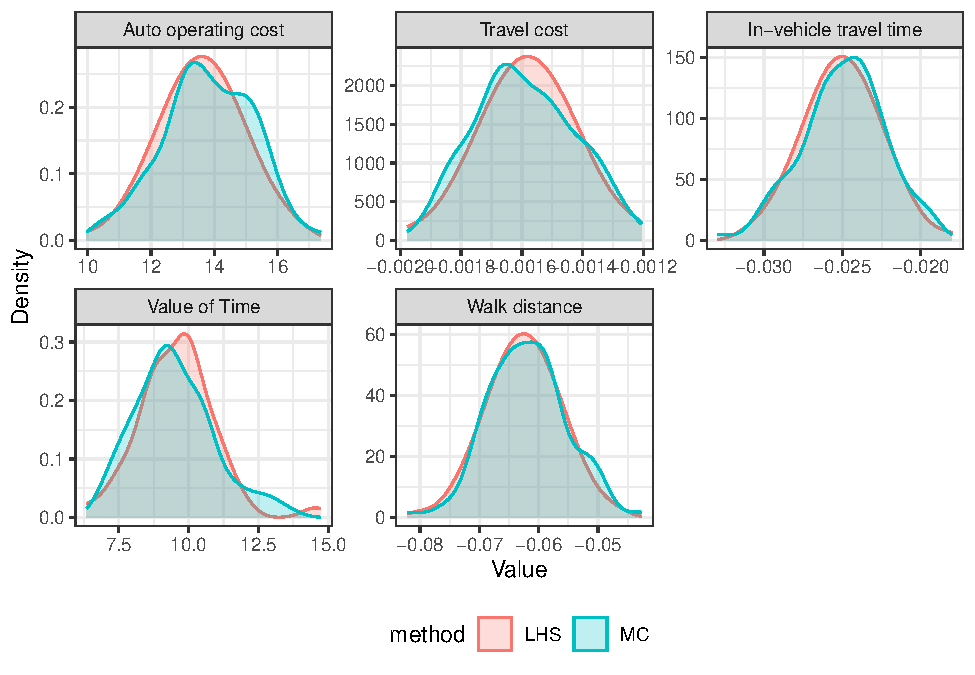
\includegraphics[width=0.8\linewidth]{thesis_files/figure-latex/parameter100-1} 

}

\caption{HBW distributions for input parameters with 100 draws.}\label{fig:parameter100}
\end{figure}

\begin{figure}

{\centering 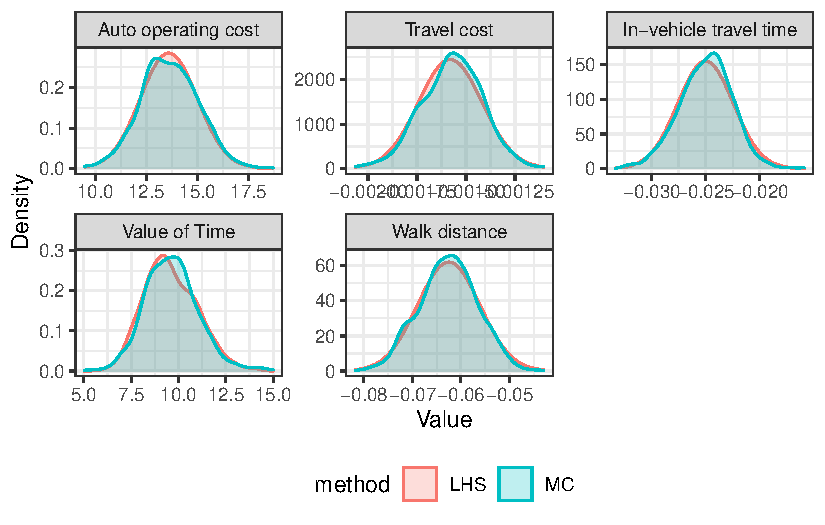
\includegraphics[width=0.8\linewidth]{thesis_files/figure-latex/parameter600-1} 

}

\caption{HBW distributions for input parameters with 600 draws.}\label{fig:parameter600}
\end{figure}

To determine if LHS is effective at a reasonable amount of iterations, the standard deviation was calculated for each additional draw. This value shows how much the mean mode choice logsum value for all zones can vary. When the standard deviation for the draws stabilizes, that shows that the amount of generated parameters has captured all of the possible variances of the results. This can be visualized for each purpose. The HBW results for the cumulative standard deviation are shown in \ref{fig:hbwstats}. The results for the other two purposes (HBO and NHB) are in \ref{fig:hbostats} and \ref{fig:nhbstats} respectively.

\begin{figure}

{\centering 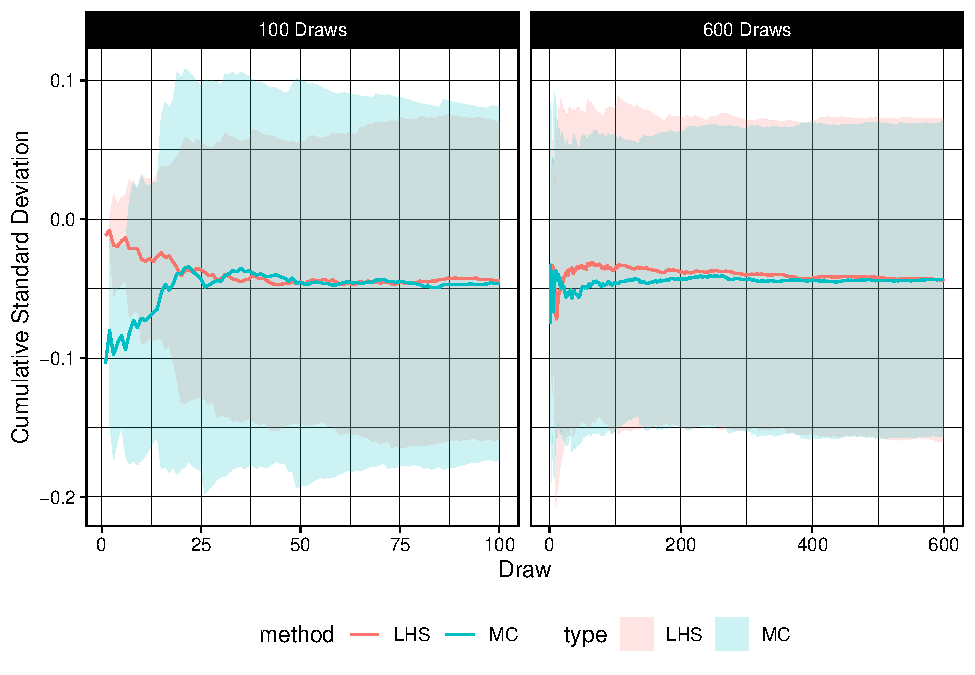
\includegraphics[width=0.8\linewidth]{thesis_files/figure-latex/hbwstats-1} 

}

\caption{HBW mean logsum standard variation with 100 and 600 draws.}\label{fig:hbwstats}
\end{figure}

\begin{figure}

{\centering 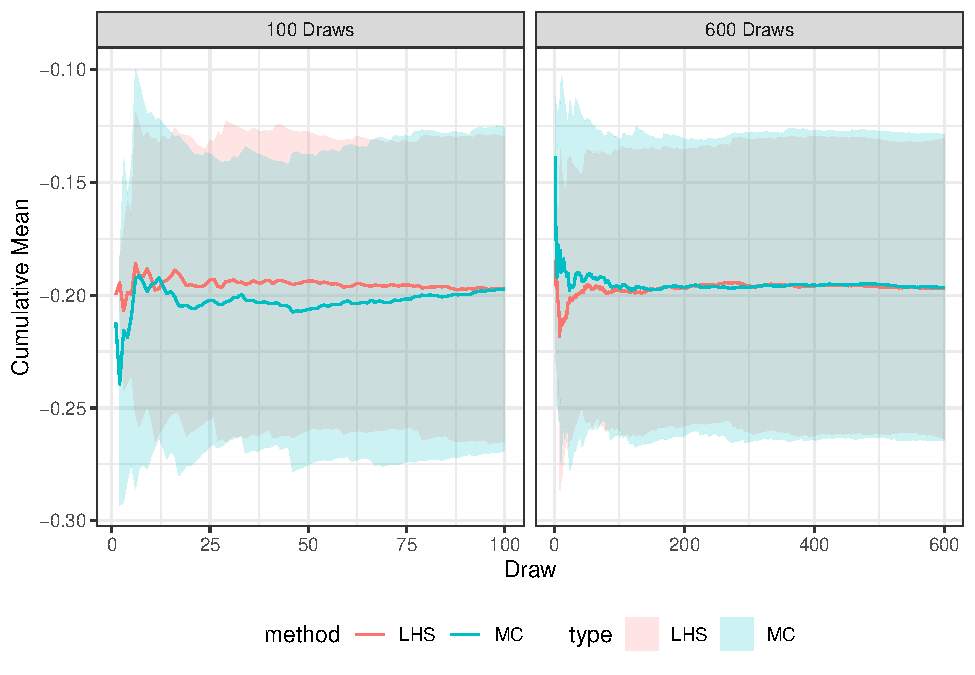
\includegraphics[width=0.8\linewidth]{thesis_files/figure-latex/hbostats-1} 

}

\caption{HBO mean logsum standard variation with 100 and 600 draws.}\label{fig:hbostats}
\end{figure}

\begin{figure}

{\centering 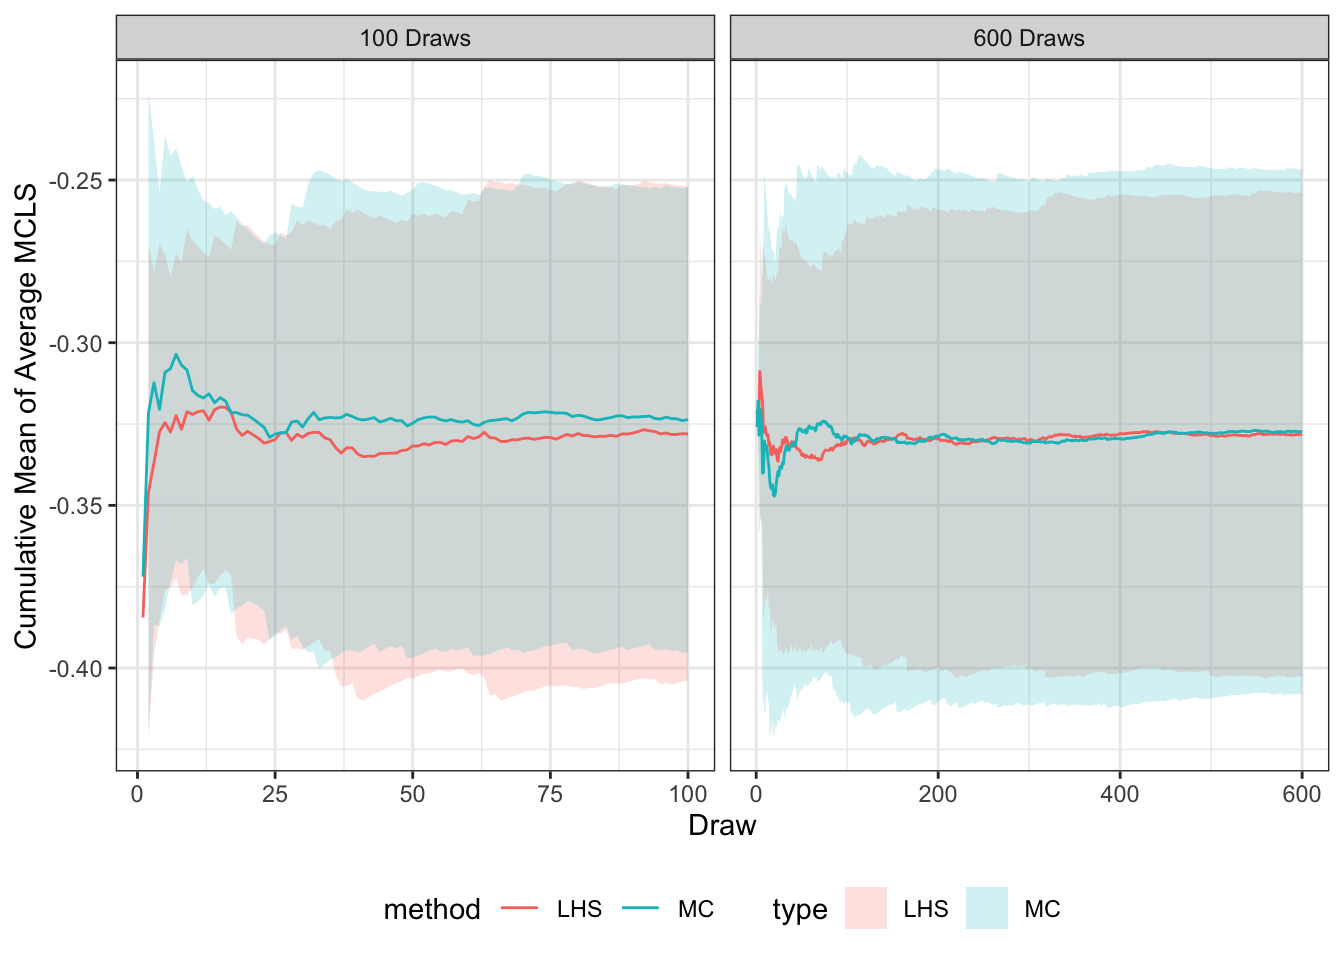
\includegraphics[width=0.8\linewidth]{thesis_files/figure-latex/nhbstats-1} 

}

\caption{NHB mean logsum standard variation with 100 and 600 draws.}\label{fig:nhbstats}
\end{figure}

For all three trip purposes, the LHS method had its standard deviation stabilized by 100 draws. The MC method had still not stabilized to the same extent after 600 draws. This shows us that Latin hypercube sampling greatly decreases the iterations needed to approximate random sampling methods. Since LHS captures the possible variance at a small enough amount of iterations, it can be used for large transportation demand models. From these results it was decided to use 100 LHS samples parameters to evaluate uncertainty within each step of the model.

\hypertarget{summary-1}{%
\section{Summary}\label{summary-1}}

A standard four-step model was created in R and CUBE to create trips, assign network volumes, and evaluate sampling methodologies. The four step model includes trip generation, trip distribution, mode and destination choice, and trip assignment. This model can be used to quantify and evaluate the uncertainty within the model using 100 draws of Latin hypercube sampling.

\hypertarget{sensitivity-analysis-results}{%
\chapter{Sensitivity Analysis Results}\label{sensitivity-analysis-results}}

\hypertarget{overview-2}{%
\section{Overview}\label{overview-2}}

Each of the 100 parameter draws was applied to the RVTPO model, generating mode choice utilities, destination choice utilities, and trip matrices for each draw. The resulting uncertainty can then be quantified using these outputs, using trips by mode and link volume.

\hypertarget{mode-choice-trips}{%
\section{Mode Choice Trips}\label{mode-choice-trips}}

Uncertainty can first be visualized by looking at how mode choices change. The total number of trips by purpose are fixed, but varies among mode type. Table \ref{tab:MCtrips} lists the base trip amount by mode and purpose. It also lists the the average number of trips across all 100 iterations, with the corresponding standard deviation and coefficient of variation. For HBW there are 103,320 auto trips. Across all 100 iterations there is a mean value of 103,298 trips with a standard deviation of 527.07. This results in a coefficient of variation of 0.0052 or 0.52\% variation in the number of auto trips. The other modes of transportation and purposes are included. The results listed in the table show that the variation of the output trips - by mode and purpose - are less than the input variation (as all COVs are smaller than 0.10). This confirms previous research that the outcome variance is less than or near the parameters variance (Clay \& Johnston, 2005; Zhao \& Kockelman, 2002). Another notable finding that can be seen in Table \ref{tab:MCtrips} is that there is greater confidence in auto trips than non-motorized or transit trips. In all three purposes that were evaluated, the coefficient of variation in auto trips are lower than transit or non-motorized trips, meaning that there is greater confidence in the models accuracy to generate auto trips. The input parameter variability has a smaller effect on auto trips than on trips on the other modes.

\begin{table}

\caption{\label{tab:MCtrips}Coefficient of Variation of Trips by Mode}
\centering
\begin{tabular}[t]{lrrrr}
\toprule
 & Base & Mean & SD & COV\\
\midrule
\addlinespace[0.3em]
\multicolumn{5}{l}{\textbf{HBW}}\\
\hspace{1em}Auto & 103320 & 103298 & 537.07 & 0.0052\\
\hspace{1em}Non-Motorized & 1103 & 1105 & 50.38 & 0.0456\\
\hspace{1em}Transit & 13254 & 13274 & 566.01 & 0.0426\\
\addlinespace[0.3em]
\multicolumn{5}{l}{\textbf{HBO}}\\
\hspace{1em}Auto & 250489 & 250475 & 453.11 & 0.0018\\
\hspace{1em}Non-Motorized & 4310 & 4316 & 235.24 & 0.0545\\
\hspace{1em}Transit & 9276 & 9283 & 363.09 & 0.0391\\
\addlinespace[0.3em]
\multicolumn{5}{l}{\textbf{NHB}}\\
\hspace{1em}Auto & 60212 & 60209 & 78.28 & 0.0013\\
\hspace{1em}Non-Motorized & 736 & 737 & 35.77 & 0.0485\\
\hspace{1em}Transit & 1576 & 1579 & 74.89 & 0.0474\\
\bottomrule
\end{tabular}
\end{table}

The variation among mode choices can be visualized graphically using a density of a scaled change in trips by mode. Figure \ref{fig:modechoicetrips} shows density plots for HBW trips by mode for twelve zones -- the zones are divided into three volume categories: low is less than 200 trips per zone, mid is 200 to 700 trips per zone, and top is greater than 700 trips per zone -- and four zones are randomly selected from each volume category. Zones that do not have any transit accessibility have been excluded. Those zones have very high density in auto trips as with the ability to choose transit was removed, the choice to choose auto was more certain. The zones included in Figure \ref{fig:modechoicetrips} all have greater certainty in auto trips, as the change in trips across all 100 iterations is relatively small. This reinforces the previous claim that the model has more confidence in auto trips than the other modes. It is also important to note that the modes are correlated to each other. In zones with a greater confidence in one mode, the other modes are more confident as well. Since the number of trips by origin zone are held constant, when there is an increase in trips on one mode there must be a decrease in trips on one or both of the other modes. Also, the distribution of non-motorized trips is similar for every zone. Suggesting that generally, the most uncertain mode is non-motorized trips, which is also verified using Table \ref{tab:MCtrips}.

\begin{sidewaysfigure}

{\centering 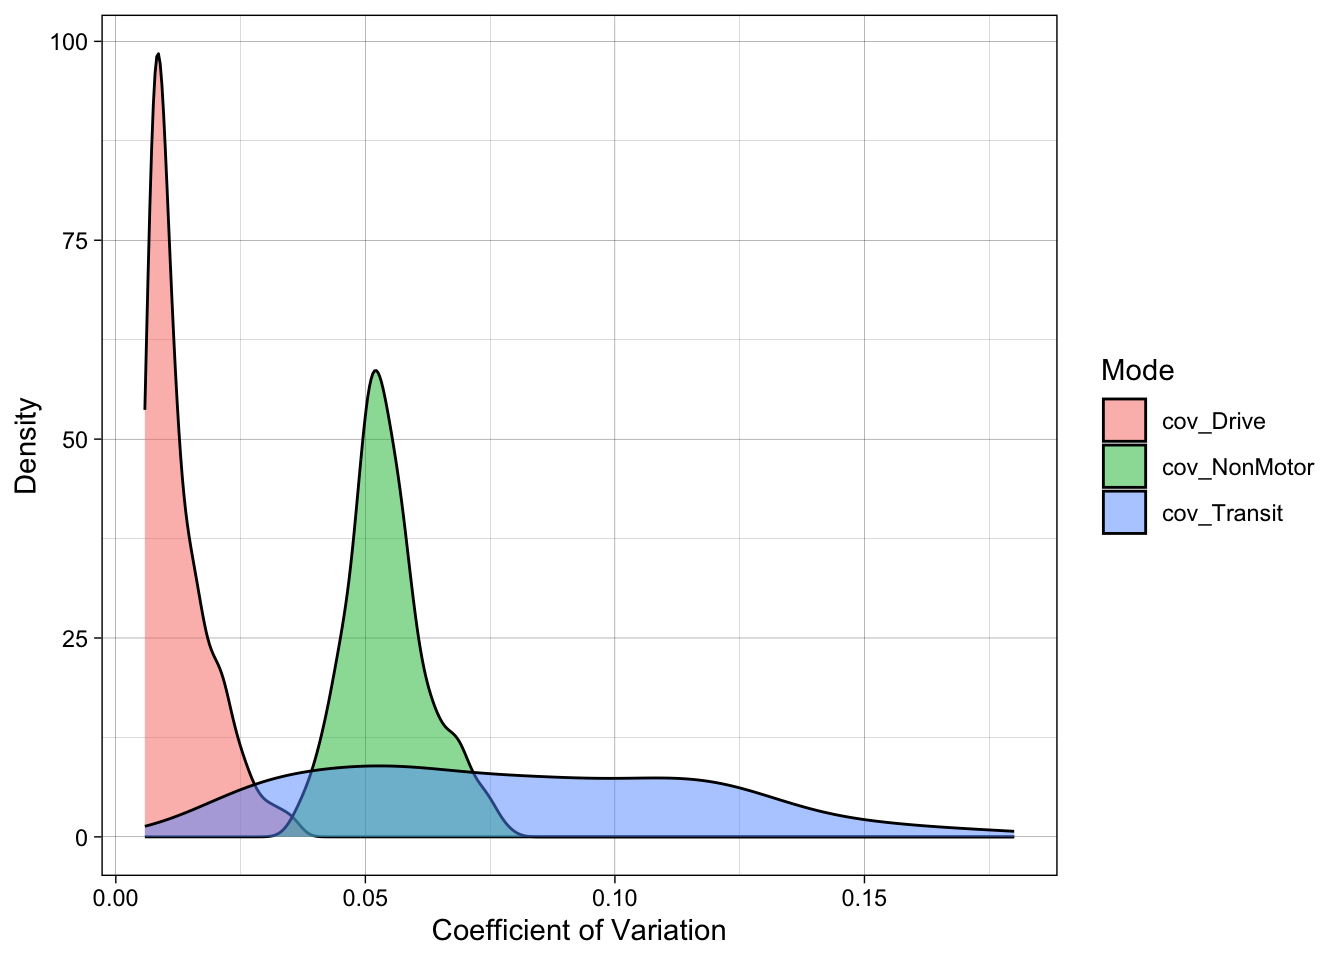
\includegraphics{thesis_files/figure-latex/modechoicetrips-1} 

}

\caption{Trip desnity for coefficient of variation by mode for HBW trips.}\label{fig:modechoicetrips}
\end{sidewaysfigure}

\hypertarget{link-volume}{%
\section{Link Volume}\label{link-volume}}

Another way to visualize uncertainty is by looking at how assigned link volume varies across iterations. Figure \ref{fig:networksd} displays variation in forecasted link volume spatially. This shows that the links with the highest standard deviation in forecasted volume are high-volume roads including freeways and principal arterials where the majority of traffic is internal to the study region. Although these links have the largest standard deviation, when compared to the total volume of the road, the variation is in reality very small. A standard deviation of 400 vehicles on a road with 40,000 total vehicles corresponds to a small variation (1\%).

\begin{sidewaysfigure}

{\centering 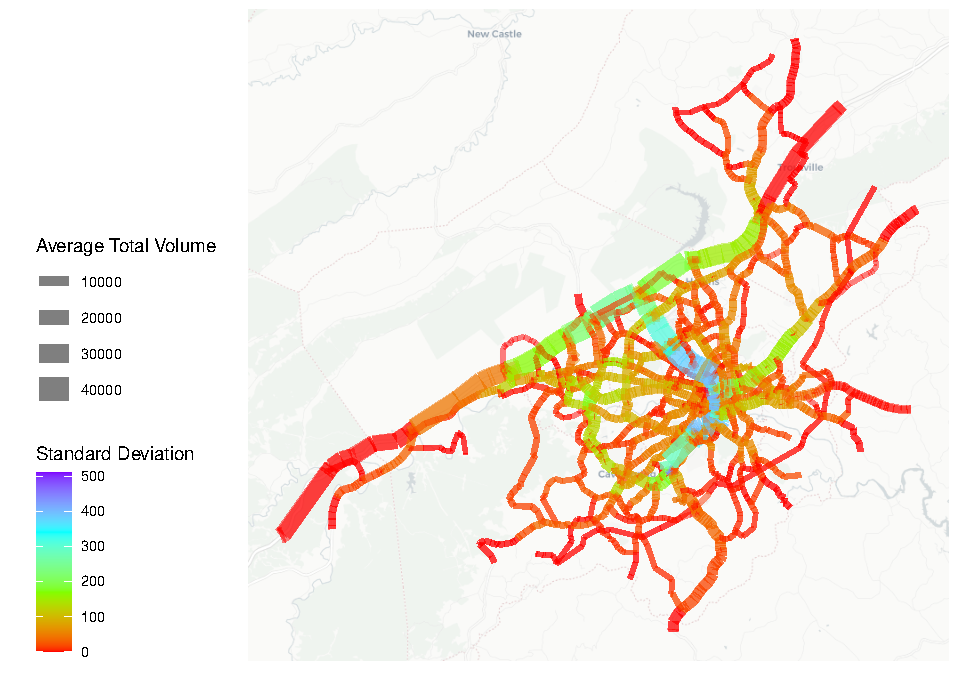
\includegraphics{thesis_files/figure-latex/networksd-1} 

}

\caption{Standard deviation in forecasted volume.}\label{fig:networksd}
\end{sidewaysfigure}

The highway assignment results can be grouped by facility type to show how the coefficient of variation compares to link volume. Figure \ref{fig:totalvolume} shows the coefficient of variation for the daily volume assigned to each network link, across the 100 draws, plotted against the mean forecasted link volume for each link. The results suggest that for high-volume roads such as major arterials and freeways, the coefficient of variation converges to approximately 0.01, or about 1\% of the road's total forecasted volume. For lower-volume links, the coefficient of variation is more widely distributed, with some local roads and small collectors having considerably higher values. Some links in the model show no variation at all; these are presumably links near the edges of the model region where the only traffic is to and from external zones, trips which were held constant in this framework.

\begin{figure}

{\centering 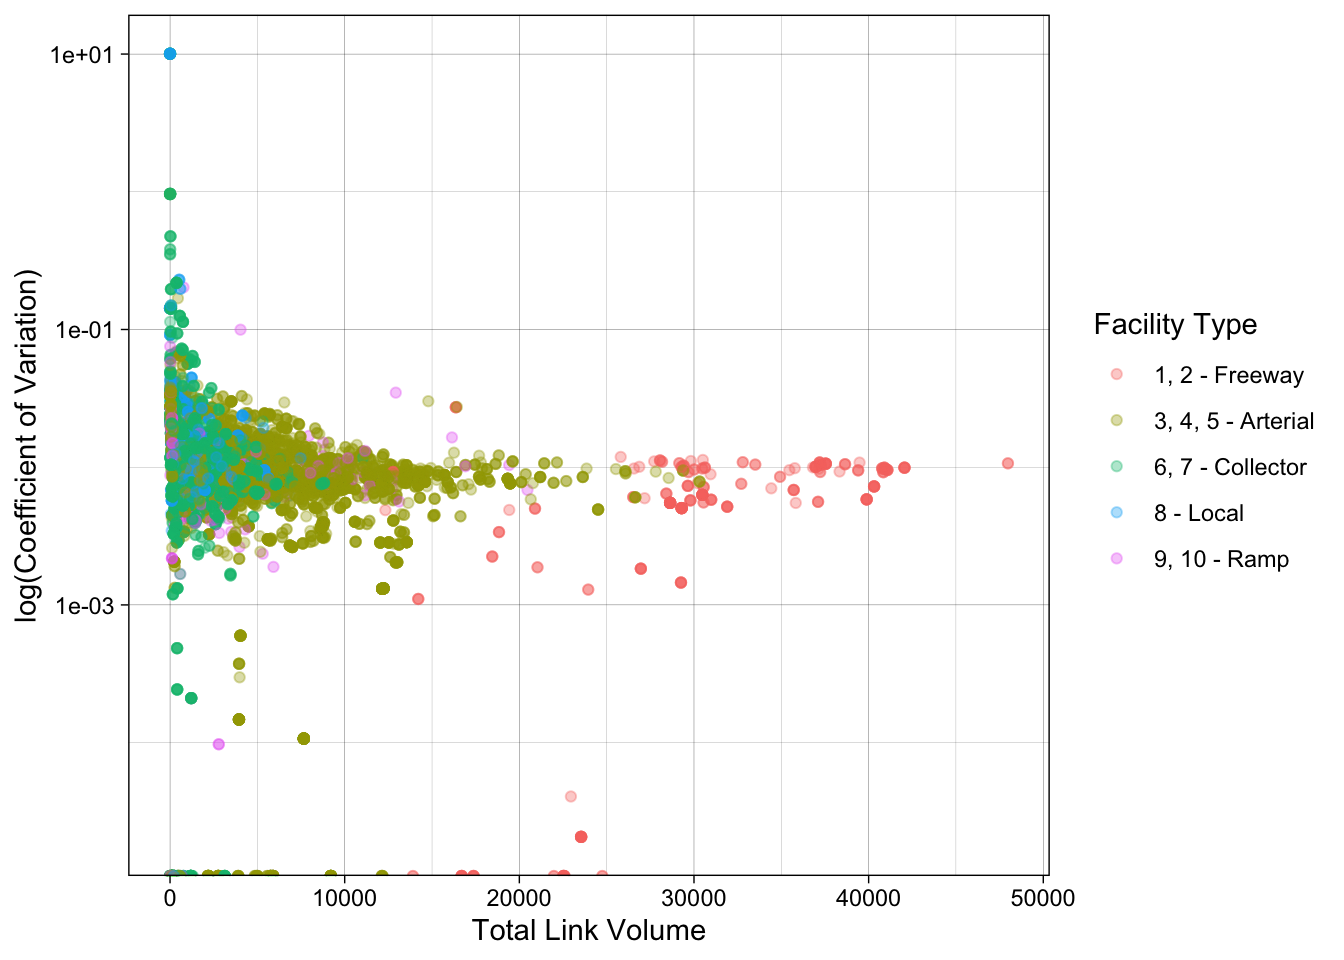
\includegraphics[width=0.8\linewidth]{thesis_files/figure-latex/totalvolume-1} 

}

\caption{Coefficient of variation in daily volume links.}\label{fig:totalvolume}
\end{figure}

Variation among a link can also be visualized with a density plot of the total volume across all iterations, as shown in Figure \ref{fig:densityplots}. In this plot, the density of forecasted volumes in three randomly selected links in each of the freeway, collector, and arterial functional types are plotted alongside the baseline forecast and the AAWDT measured by the Virginia Department of Transportation, and to which the model estimates were calibrated. In all cases, the error or uncertainty in the forecast is considerably narrower than the error inherent in the model construction, as evidenced by the fact that the AAWDT target value is well outside the bell curve created the statistically varied simulation forecasts.

As expected from using the base parameter values as the mean of the LHS parameter sampling, the base results are at or near the median of the statistical density for each link's volume. But it is notable that the estimated volumes are not perfectly, normally distributed as might be naively expected. In this case, the combined effects of the mode and destination choice parameter sampling appear to be constrained by the geographic specificity of the RVTPO model network: even when the demand for trips changes between zone pairs, the realities of the highway capacity, volume-delay, and static user equilibrium procedures may be limiting the possibilities for forecasted highway volumes.

\begin{sidewaysfigure}

{\centering 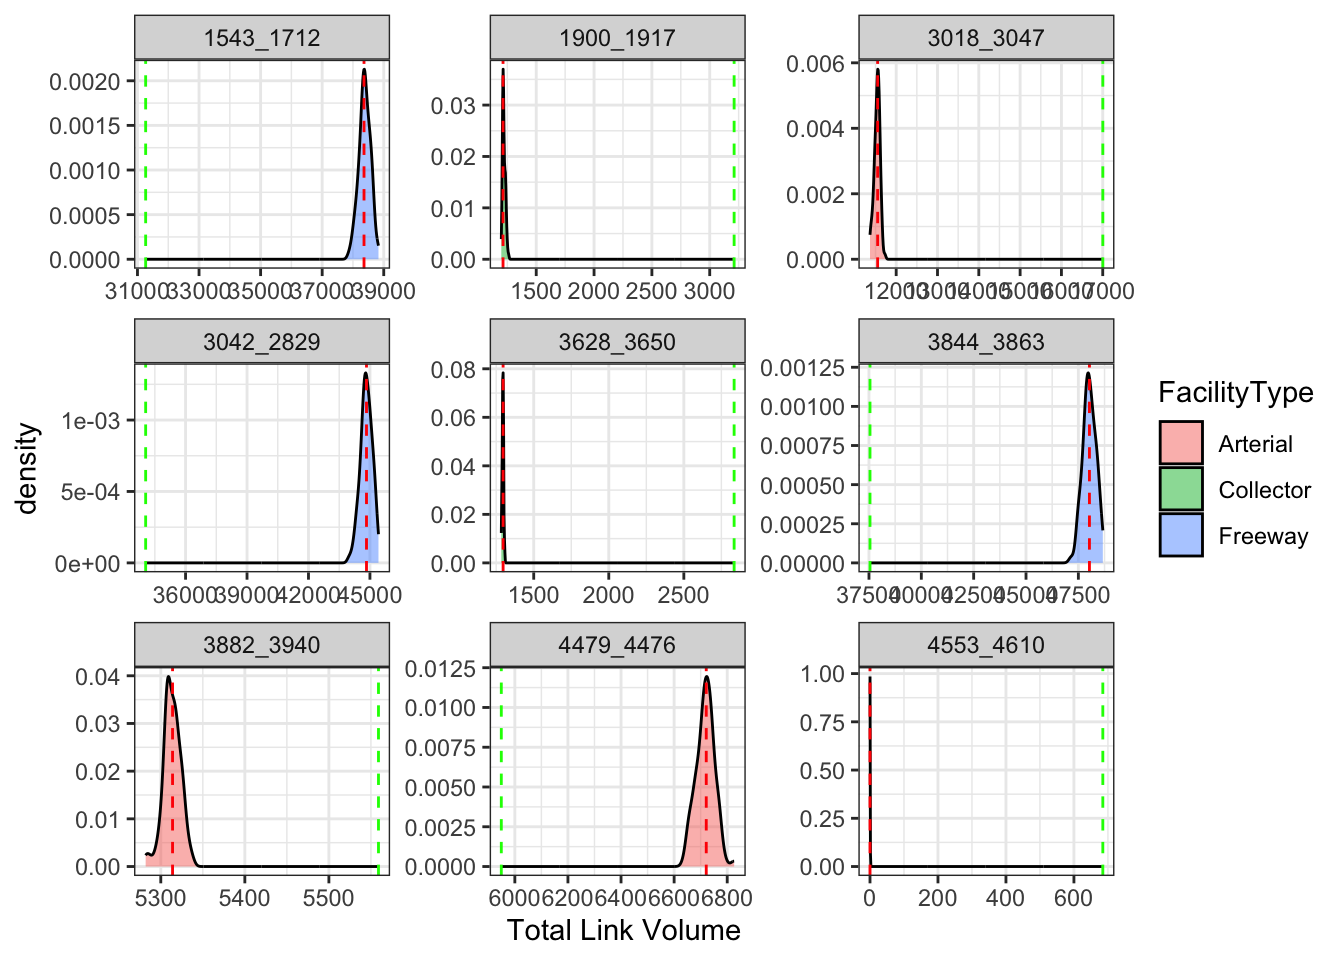
\includegraphics{thesis_files/figure-latex/densityplots-1} 

}

\caption{Density plot of forecasted volume on selected links, with default parameter results marked in red, and AAWDT values in green.}\label{fig:densityplots}
\end{sidewaysfigure}

\hypertarget{summary-2}{%
\section{Summary}\label{summary-2}}

The uncertainty and variance present in the model results are overall smaller than the variability introduced to the model through the parameters. Auto trips are more certain than transit or non-motorized trips, regardless of the amount of trips in a given zone. When there is only two modes available auto trips are even more certain. Higher volume roads have greater certainty than lower volume ones. Also, uncertainty that exists within the first three steps of the model appears to be corrected by the limitations of the highway network assignment.

\hypertarget{conclusions}{%
\chapter{Conclusions}\label{conclusions}}

\hypertarget{overview-3}{%
\section{Overview}\label{overview-3}}

In general, this research has shown that statistical parameter uncertainty does not appear to be a significant factor in forecasting traffic volumes using transportation demand models. The result uncertainty is generally equally to or smaller than the input parameter variance. The described model is most confident in auto trip distributions, and on higher volume facilities. Any variation in mode and destination choice probabilities appears to be corrected by the limitations of the highway network assignment.

\hypertarget{limitations-and-further-research}{%
\section{Limitations and Further Research}\label{limitations-and-further-research}}

There are several limitations that must be mentioned in this research, however. First, we did not attempt to address the statistical uncertainty in trip rate estimates; these may play a substantially larger role than destination and mode choice parameters, given that lower trip rates may lead to lower traffic volumes globally, which could not be ``corrected'' by the static user equilibrium assignment. And the assignment itself might have been aided in this case by the RVTPO's relatively simplistic highway network: if only two major interstates exist the number of realistic lowest cost path choices between regions is somewhat constrained. It may be that in a larger network with more path redundancies, the assignment may not have been as helpful in constraining the forecasted volumes.

In this research we had only the estimates of the statistical coefficients, and therefore had to assume a coefficient of variation to derive variation in the sampling procedure. It would be better if model user and development documentation more regularly provided estimates of the standard errors of model parameters. Even better would be variance-covariance matrices for the estimated models, enabling researchers to ensure that covariance relationships between sampled parameters are maintained. The parameters were also varied without respect to the other parameters. The parameters are often related to one another, additional research should be done to see how an increase in correlated parameters effect the model results.

\hypertarget{summary-3}{%
\section{Summary}\label{summary-3}}

Notwithstanding these limitations, statistical parameter variance is not likely the largest source of uncertainty in travel forecasting. There are likely more important factors at play that planners and government agencies should address. Research on all sources of uncertainty is somewhat limited, but in many ways has been hampered by the burdensome computational requirements of many modern travel models (Voulgaris, 2019). This research methodology benefited from a lightweight travel model that could be repeatedly re-run with dozens of resampled choice parameters. Better understanding the other sources of uncertainty -- model specification and input accuracy -- might also benefit from lightweight models constructed for transparency and flexibility rather than heavily constrained models emphasizing precise spatial detail and strict behavioral constraints. This might allow forecasts to be made with an ensemble approach (Wu \& Levinson, 2021), identifying preferred policies as the consensus of multiple plausible model specifications.

\hypertarget{references}{%
\chapter*{References}\label{references}}
\addcontentsline{toc}{chapter}{References}

\pagestyle{myrefs}

\hypertarget{refs}{}
\begin{CSLReferences}{1}{0}
\leavevmode\vadjust pre{\hypertarget{ref-armoogum2009measuring}{}}%
Armoogum, J., Madre, J.-L., \& Bussiere, Y. (2009). Measuring uncertainty in long-term travel demand forecasting from demographic modelling: Case study of the paris and montreal metropolitan areas. \emph{IATSS Research}, \emph{33}(2), 9--20.

\leavevmode\vadjust pre{\hypertarget{ref-clay2005univariate}{}}%
Clay, M. J., \& Johnston, R. A. (2005). Univariate uncertainty analysis of an integrated land use and transportation model: MEPLAN. \emph{Transportation Planning and Technology}, \emph{28}(3), 149--165.

\leavevmode\vadjust pre{\hypertarget{ref-duthie2010highway}{}}%
Duthie, J., Voruganti, A., Kockelman, K., \& Waller, S. T. (2010). Highway improvement project rankings due to uncertain model inputs: Application of traditional transportation and land use models. \emph{Journal of Urban Planning and Development}, \emph{136}(4), 294--302.

\leavevmode\vadjust pre{\hypertarget{ref-flyvbjerg2005accurate}{}}%
Flyvbjerg, B., Skamris Holm, M. K., \& Buhl, S. L. (2005). How (in) accurate are demand forecasts in public works projects?: The case of transportation. \emph{Journal of the American Planning Association}, \emph{71}(2), 131--146.

\leavevmode\vadjust pre{\hypertarget{ref-helton2003latin}{}}%
Helton, J. C., \& Davis, F. J. (2003). Latin hypercube sampling and the propagation of uncertainty in analyses of complex systems. \emph{Reliability Engineering \& System Safety}, \emph{81}(1), 23--69.

\leavevmode\vadjust pre{\hypertarget{ref-hoque2021estimating}{}}%
Hoque, J. M., Erhardt, G. D., Schmitt, D., Chen, M., \& Wachs, M. (2021). Estimating the uncertainty of traffic forecasts from their historical accuracy. \emph{Transportation Research Part A: Policy and Practice}, \emph{147}, 339--349.

\leavevmode\vadjust pre{\hypertarget{ref-koppelman2006self}{}}%
Koppelman, F. S., \& Bhat, C. (2006). \emph{A self instructing course in mode choice modeling: Multinomial and nested logit models}.

\leavevmode\vadjust pre{\hypertarget{ref-manzo2015uncertainty}{}}%
Manzo, S., Nielsen, O. A., \& Prato, C. G. (2015). How uncertainty in input and parameters influences transport model: Output a four-stage model case-study. \emph{Transport Policy}, \emph{38}, 64--72.

\leavevmode\vadjust pre{\hypertarget{ref-national2012travel}{}}%
National Academies of Sciences, Engineering, Medicine, et al. (2012). \emph{Travel demand forecasting: Parameters and techniques}.

\leavevmode\vadjust pre{\hypertarget{ref-petrik2020uncertainty}{}}%
Petrik, O., Adnan, M., Basak, K., \& Ben-Akiva, M. (2020). Uncertainty analysis of an activity-based microsimulation model for singapore. \emph{Future Generation Computer Systems}, \emph{110}, 350--363.

\leavevmode\vadjust pre{\hypertarget{ref-petrik2016measuring}{}}%
Petrik, O., Moura, F., \& Silva, J. de A. e. (2016). Measuring uncertainty in discrete choice travel demand forecasting models. \emph{Transportation Planning and Technology}, \emph{39}(2), 218--237.

\leavevmode\vadjust pre{\hypertarget{ref-rasouli2012uncertainty}{}}%
Rasouli, S., \& Timmermans, H. (2012). Uncertainty in travel demand forecasting models: Literature review and research agenda. \emph{Transportation Letters}, \emph{4}(1), 55--73.

\leavevmode\vadjust pre{\hypertarget{ref-rodier2002uncertain}{}}%
Rodier, C. J., \& Johnston, R. A. (2002). Uncertain socioeconomic projections used in travel demand and emissions models: Could plausible errors result in air quality nonconformity? \emph{Transportation Research Part A: Policy and Practice}, \emph{36}(7), 613--631.

\leavevmode\vadjust pre{\hypertarget{ref-voulgaris2019crystal}{}}%
Voulgaris, C. T. (2019). Crystal balls and black boxes: What makes a good forecast? \emph{Journal of Planning Literature}, \emph{34}(3), 286--299.

\leavevmode\vadjust pre{\hypertarget{ref-welde2011planners}{}}%
Welde, M., \& Odeck, J. (2011). Do planners get it right? The accuracy of travel demand forecasting in norway. \emph{European Journal of Transport and Infrastructure Research}, \emph{11}(1).

\leavevmode\vadjust pre{\hypertarget{ref-wu2021ensemble}{}}%
Wu, H., \& Levinson, D. (2021). The ensemble approach to forecasting: A review and synthesis. \emph{Transportation Research Part C: Emerging Technologies}, \emph{132}, 103357.

\leavevmode\vadjust pre{\hypertarget{ref-yang2013sensitivity}{}}%
Yang, C., Chen, A., Xu, X., \& Wong, S. (2013). Sensitivity-based uncertainty analysis of a combined travel demand model. \emph{Transportation Research Part B: Methodological}, \emph{57}, 225--244.

\leavevmode\vadjust pre{\hypertarget{ref-zhao2002propagation}{}}%
Zhao, Y., \& Kockelman, K. M. (2002). The propagation of uncertainty through travel demand models: An exploratory analysis. \emph{The Annals of Regional Science}, \emph{36}(1), 145--163.

\end{CSLReferences}

\cleardoublepage
\pagestyle{byu}

%%%%%%%%%%%%%%%%%%%%%%%%
% --- Bibliography --- %
%%%%%%%%%%%%%%%%%%%%%%%%
% printed automatically with CSL
%
%%%%%%%%%%%%%%%%%%%%%
% --- Appendices --- %
%%%%%%%%%%%%%%%%%%%%%


\end{document}
